\documentclass[12pt]{article}
\usepackage{ctex}
\usepackage{geometry}
\usepackage{amsmath}
\usepackage{graphicx}
\usepackage{minted}
\setlength{\parskip}{0.3\baselineskip}
\setlength{\parindent}{2em}
\begin{document}
\title{NOIP2017模拟题}
\author{XLightGod}
\maketitle
\begin{center}

考试时限:5h

\begin{tabular}{|l|p{100pt}|p{100pt}|p{100pt}|}
    \hline
    题目名称&小Y&暗牧&大根\\ \hline
    输入文件名&y.in&m.in&dagon.in\\ \hline
    输出文件名&y.out&m.out&dagon.out\\ \hline
    测试点数目&$10$&$10$&$20$\\ \hline
    时限&$1s$&$2s$&$1s$\\ \hline
    内存限制&$256MB$&$256MB$&$256MB$\\ \hline
\end{tabular}
\end{center}

题目简单,请认真对待。

如果你发现原题,请不要声张;如果你AK了,请不要提前交卷。

评测开启O2优化与无限栈。所有部分分均以subtask的形式给出。

如机器配置有较大差异,时限可调整为标程的 $1.5$ 倍。

题目难度顺序可能非题目顺序。

\newpage

\section{小Y(y)}
\subsection{题目描述}

小Y有一个 $1$ 到 $N$ 的排列 $P$ 。有 $M$ 个询问,每个询问给定 $4$ 个整数 $l_1,r_1,l_2$ 和$r_2(1\le l_1\le r_1<l_2\le r_2\le N,r_1-l_1=r_2-l_2)$ 。你需要回答有多少长度为 $S=r_1−l_1+1$ 的排列 $Q$ 满足:

$$P_{Q_i+l_1−1}<P_{i+l_2−1},\forall 1\le i\le S$$

请你帮小Y求出每个询问的方案数对 $10^9+7$ 取模的结果。

\subsection{输入格式}

输入的第一行包含一个整数 $T$ ,表示测试数据的组数。

每组数据的第一行包含两个整数 $N$ 和 $M$ 。接下来一行包含 $N$ 个整数 $P_1,P_2,...,P_N$ 。接下来 $M$ 行,每行包含 $4$ 个整数 $l_1,r_1,l_2$ 和 $r_2$ ,代表一个询问。

\subsection{输出格式}

对于每个询问,输出一行,包含一个整数,代表方案数对 $10^9+7$ 取模得到的结果。

\subsection{样例输入}

\begin{minted}{c++}
3
4 1
1 2 3 4
1 2 3 4
4 2
1 3 2 4
1 1 2 2
1 2 3 4
10 1
1 4 3 2 9 5 6 7 10 8
1 5 6 10
\end{minted}

\subsection{样例输出}

\begin{minted}{c++}
2
1
1
24
\end{minted}

\subsection{数据范围}

对于 $10\%$ 的数据, $N\le 10$ 。

对于 $30\%$ 的数据, $N\le 1000$ 。

对于 $100\%$ 的数据,

$1\le T\le 10$ ,

$1\le$ 输入中每组数据的 $N$ 之和 $\le 10^5$ ,

$1\le$ 输入中每组数据的 $M$ 之和 $\le 10^5$ ,

$0\le$ 排列 $P$ 的逆序对数 $\le 10^5$ 。

\newpage
\section{暗牧(m)}
\subsection{题目描述}

在Dato3的世界里,英雄们通过对量子力学的研究,发现了世界上其实存在着无数个位面——即是也被称作平行宇宙的存在。

位面有无数多个,每个位面中包含 $n$ 颗行星,由 $n−1$ 个虫洞链接。同一个位面中的任意两颗行星间有唯一的虫洞路径。

量子力学之父巴拉森指出:“每个位面都看起来差不多。”,揭示了所有位面中的虫洞都是相同的的道理。也即,如果某个位面中在行星 $q_1$ 和 $q_2$ 之间有虫洞,那么任意位面中 $q_1$ 和 $q_2$ 间都有虫洞。位面从 $1$ 开始编号,一个位面中的行星编号为 $1$ 到 $n$ 。因此使用位面和行星的编号就能唯一确定一颗行星。

艾欧使用它最近获得的至宝"Portal Gun"建造了 $m$ 个可以双向通行的传送门。每个传送门用四个整数 $p_1,u_1,p_2,u_2$ 描述,代表可以让人们在 $u_1$ 位面的 $p_1$ 行星和 $u_2$ 位面的 $p_2$ 行星间移动。通过虫洞或者传送门移动都需要花费 $1$ 单位的时间。

负责星际医疗协助的暗影牧师戴泽希望你能帮忙计算行星间的最短路,共有 $q$ 个询问需要你回答。

\subsection{输入格式}

输入的第一行包含三个整数 $n,m$ 和 $q$ ,分别代表单个位面中的行星数、传送门的数量,以及询问的数量。

接下来 $n−1$ 行描述位面中的虫洞,每行包含两个整数,代表一个虫洞所连接的两个行星。

接下来 $m$ 行描述传送门,每行包含四个整数 $p_1,u_1,p_2,u_2$ 。

接下来 $q$ 行描述询问,每行包含四个整数 $p_1,u_1,p_2,u_2$ ,你需要回答从 $u_1$ 位面的 $p_1$ 行星到 $u_2$ 位面的 $p_2$ 行星的最短距离。

\subsection{输出格式}

对于每个询问,输出一行,包含一个整数,代表最短路径的耗时。如果无法到达,则输出“impossible”(不含引号)。

\subsection{样例输入}

\begin{minted}{c++}
3 3 3
1 2
2 3
1 1 1 3
3 1 3 2
1 2 3 3
2 1 2 2
2 1 2 3
1 2 3 2
\end{minted}

\subsection{样例输出}

\begin{minted}{c++}
3
4
2
\end{minted}

\subsection{数据范围}

对于 $30\%$ 的数据, $1\le n\le 1000,1\le m\le 3000,1\le u1,u2\le 1000$ 。

对于另外 $20\%$ 的数据,一个位面中的行星形成一条链。

对于 $100\%$ 的数据, $1\le n\le 300000,1\le m\le 100000,1\le q\le 10,1\le p1,p2\le n,1\le u1,u2\le 200000$ 。

保证由虫洞和传送门形成的整张图不含重边或自环。

\newpage
\section{大根(dagon)}
\subsection{题目描述}

作为瘟疫法师的喜爱者,他对自己的胜率不是很满意。

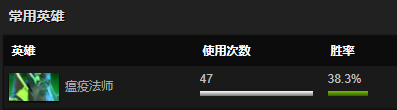
\includegraphics[width=0.6\textwidth]{nec.png}

为了让自己变得更加强大,他踏上了寻找神器——达贡之神力(大根)的道路。

历经千辛万苦后,他终于打败了达贡,得到了达贡之神力。然而,达贡对他说:“其实,这并不是这根法杖的最终形态。我得到它之后,一直被这根法杖上的难题所困扰。如果你能解开这道难题,就能解放它的真正力量。”

“法杖上有 $n$ 条沿法杖方向的纹路,你可以认为这些纹路是以整根法杖为数轴上的一个个区间。你需要将 $k$ 种元素注入这些纹路,每一条纹路中只能且必须注入一种元素。”

“某一种元素提供的能量为该元素注入的所有纹路代表区间的交的长度。如果你能使所有元素提供的能量达到最大,就可以激活这根法杖。”

被胜利的喜悦冲昏头脑的他已经思考不清这样的题目了。现在,他请你帮助他解决这个难题。

\subsection{输入格式}

第一行两个正整数 $n,k$ 。

接下来 $n$ 行,第 $i$ 行两个整数 $l_i,r_i$ ,表示第 $i$ 条纹路所对应的区间的两个端点。

\subsection{输出格式}

一行一个整数表示最大能量。

\subsection{样例输入}

\begin{minted}{c++}
5 3
5 10
4 11
6 9
10 30
20 40
\end{minted}

\subsection{样例输出}

\begin{minted}{c++}
43
\end{minted}

\subsection{样例解释}

将第一种元素注入前三条纹路,其余两种元素分别注入后两条纹路。

前三条纹路代表区间的交为 $[6,9]$ ,提供 $3$ 点能量;其余两种元素各提供 $20$ 点能量。

\subsection{数据范围}

对于 $10\%$ 的数据, $n\le 8$ 。

对于 $30\%$ 的数据, $n\le 300$ 。

对于 $60\%$ 的数据, $n\le 6000$ 。

对于 $100\%$ 的数据, $1\le k\le n\le 1000000,l_i\le r_i$ 。

\end{document}
